\documentclass[acmsmall,nonacm]{acmart}

% suppress the ACM reference/copyright block
\settopmatter{printacmref=false}
\renewcommand\footnotetextcopyrightpermission[1]{}
\pagestyle{plain}

\usepackage{listings}
\usepackage{xcolor}
\usepackage{booktabs}
\usepackage{mdframed}
\usepackage{enumitem}
\usepackage{microtype}

% ---- code styles -------------------------------------------------------
\lstdefinestyle{java}{
  language=Java,
  basicstyle=\ttfamily\small,
  breaklines=true,
  frame=single,
  backgroundcolor=\color{gray!8},
  keywordstyle=\color{blue!65}\bfseries,
  commentstyle=\color{green!40!black}\itshape,
  stringstyle=\color{red!55!black},
  tabsize=4,
  captionpos=b,
  numbers=left,
  numberstyle=\tiny\color{gray},
  numbersep=5pt,
  showstringspaces=false,
}
\lstdefinestyle{shell}{
  basicstyle=\ttfamily\small,
  breaklines=true,
  frame=single,
  backgroundcolor=\color{gray!5},
  tabsize=2,
  showstringspaces=false,
}

% prompt / response boxes
\newmdenv[
  backgroundcolor=blue!4,
  linecolor=blue!25,
  roundcorner=3pt,
  innerleftmargin=9pt, innerrightmargin=9pt,
  innertopmargin=5pt,  innerbottommargin=5pt,
]{promptbox}
\newmdenv[
  backgroundcolor=green!4,
  linecolor=green!35!black,
  roundcorner=3pt,
  innerleftmargin=9pt, innerrightmargin=9pt,
  innertopmargin=5pt,  innerbottommargin=5pt,
]{responsebox}
% ------------------------------------------------------------------------

\title{COMP5111 Assignment 1 Task 3: Exploring LLM-Based Specification-Driven Test Generation}
\subtitle{Student ID: 21139878}

\author{Zimo Ji}
\email{zjiag@cse.ust.hk}
\affiliation{%
  \institution{Hong Kong University of Science and Technology}
  \country{Hong Kong SAR, China}
}

\begin{document}
\maketitle

\tableofcontents
\newpage

%% ==========================================================================
\section{Overview}
%% ==========================================================================

This report documents my exploration of using \textbf{GPT-5.2} for specification-based JUnit~4
test generation on \texttt{comp5111.assignment.cut.Subject}. Accroding to the  assignment requirements, the main idea is:
Giving the model only function signatures and docstrings (no implementation code), and see how good
the generated tests are.

I selected \textbf{15 functions} from three inner classes: \texttt{StringAlgorithms} (8~functions),
\texttt{DateTimeAlgorithms} (6), and \texttt{GamePlace} (1). Line coverage is measured using the
Soot-based tool built for Task~2, and all API calls used the OpenAI Python SDK v2.26.0 with
\texttt{max\_completion\_tokens=8000}.

\medskip\noindent\textbf{Functions tested:}
\begin{itemize}
  \item \texttt{StringAlgorithms}: \texttt{startsWithIgnoreCase}, \texttt{trimArrayElements},
        \texttt{strToBoolean} (1-param and 4-param),
        \texttt{extractIntInStr}, \texttt{getVersionNo}, \texttt{padLeft}, \texttt{parseToken}
  \item \texttt{DateTimeAlgorithms}: \texttt{calcDaysInMonth}, \texttt{judgeLeapYear},
        \texttt{roundSecondToString}, \texttt{dayStr}, \texttt{getQuarter}, \texttt{month2MonAbbr}
  \item \texttt{GamePlace}: \texttt{isAdjacent} (+ \texttt{manhattanDistance} picked up by the advanced prompt)
\end{itemize}

%% ==========================================================================
\section{Subtask 1: Test Generation from Current Specifications}
%% ==========================================================================

\subsection{Simple Prompt (Baseline)}

The baseline prompt is intentionally bare-bones: paste the docstrings, add a one-liner instruction.

\subsubsection*{Interaction Record}

\begin{promptbox}
\textbf{[USER]}\\[4pt]
Write JUnit 4 test cases for the following Java methods. Only use the method signatures and their docstrings.

\begin{verbatim}
public class Subject {
    public static class StringAlgorithms {
        /**
         * Returns true if the given string starts with the specified
         * case-insensitive prefix, false otherwise.
         * @param str    the String to check
         * @param prefix the prefix to look for
         * @return true if ... false otherwise.
         */
        public static boolean startsWithIgnoreCase(String str, String prefix);

        /**
         * Extract an integer from a string.
         * Rules:
         * null or empty string -> 0
         * 1234 -> 1234
         * a -> 0
         * 1234a123 -> 123
         * @param str a string to extract the integer.
         */
        public static int extractIntInStr(String str);

        /**
         * Parses a token until any of the specified terminator
         * characters is encountered.
         * @param str         the string to parse
         * @param terminators the array of terminating characters
         * @return the parsed token
         */
        public static String parseToken(String str, char[] terminators);

        /**
         * Converts seconds into a human-readable string representing
         * the largest time unit (years, weeks, days, hours, minutes,
         * or seconds).
         * @param sec the time in seconds to convert
         * @return a string representing the converted time
         */
        public static String roundSecondToString(long second);

        // ... (remaining 11 functions with their original docstrings)
    }
}
\end{verbatim}

Generate JUnit 4 test class, package \texttt{comp5111.assignment.cut},
class name \texttt{LLMSimpleTest}. Output only the Java code, no explanations.
\end{promptbox}

\bigskip

\begin{responsebox}
\textbf{[GPT-5.2 RESPONSE]} (excerpted key tests)

\begin{verbatim}
@Test
public void testExtractIntInStr_stopsAtFirstNonDigitAfterDigits() {
    // docstring says: 1234a123 -> 123
    assertEquals(123, Subject.StringAlgorithms.extractIntInStr("1234a123"));
    assertEquals(9, Subject.StringAlgorithms.extractIntInStr("9x9"));
}

@Test
public void testParseToken_stopsAtTerminator() {
    // "until terminator is encountered" -- LLM assumed this means excluded
    assertEquals("abc", Subject.StringAlgorithms.parseToken(
        "abc,def", new char[]{',', ';'}));
}

@Test
public void testRoundSecondToString_seconds() {
    String s = Subject.DateTimeAlgorithms.roundSecondToString(59L);
    // no output format specified, so we do a fuzzy check
    assertTrue("Should mention seconds unit",
        s.toLowerCase().contains("sec") || s.contains("S"));
}
\end{verbatim}
\end{responsebox}

\medskip

As observed, the model faithfully copied
the wrong example from the docstring (\texttt{1234a123 -> 123}) and used it as an assertion.
For \texttt{parseToken} it inferred exclusion of the terminator from the word ``until''---a
reasonable reading, but wrong. And for \texttt{roundSecondToString} it had to fall back on a
\texttt{contains("sec")} check since the docstring gives no format at all. Interestingly, the model
also tried to instantiate \texttt{GamePlace} via \texttt{new Subject().new GamePlace()} which is
technically correct, though it had to guess constructor arguments.

\subsubsection*{Execution Results}

\begin{lstlisting}[style=shell, caption={Test execution output for LLMSimpleTest}]
JUnit version 4.12
......E...................E..E..............
Time: 0.03

There were 3 failures:
1) testParseToken_terminatorFirstYieldsEmpty
   expected:<[]> but was:<[,]>
2) testExtractIntInStr_stopsAtFirstNonDigitAfterDigits
   expected:<123> but was:<1234>
3) testParseToken_stopsAtTerminator
   expected:<abc[]> but was:<abc[,]>

Tests run: 41,  Failures: 3
\end{lstlisting}

\noindent\textbf{Line coverage (Soot-based):}

\begin{table}[h]
\centering
\begin{tabular}{lrr}
\toprule
\textbf{Class} & \textbf{Total lines} & \textbf{Covered (\%)} \\
\midrule
Subject (outer)              & 1   & 100.0\% \\
Subject\$StringAlgorithms    & 197 & 105\;\;(53.3\%) \\
Subject\$DateTimeAlgorithms  & 159 & 50\;\;(31.4\%) \\
Subject\$GamePlace           & 30  & 9\;\;(30.0\%) \\
Subject\$GamePlayer          & 24  & 0\;\;(0.0\%) \\
Subject\$GameConfiguration   & 100 & 0\;\;(0.0\%) \\
\midrule
\textbf{Overall}             & \textbf{511} & \textbf{165\;\;(32.3\%)} \\
\bottomrule
\end{tabular}
\caption{LLMSimpleTest line coverage (Soot tool)}
\end{table}

\begin{figure}[h]
\centering
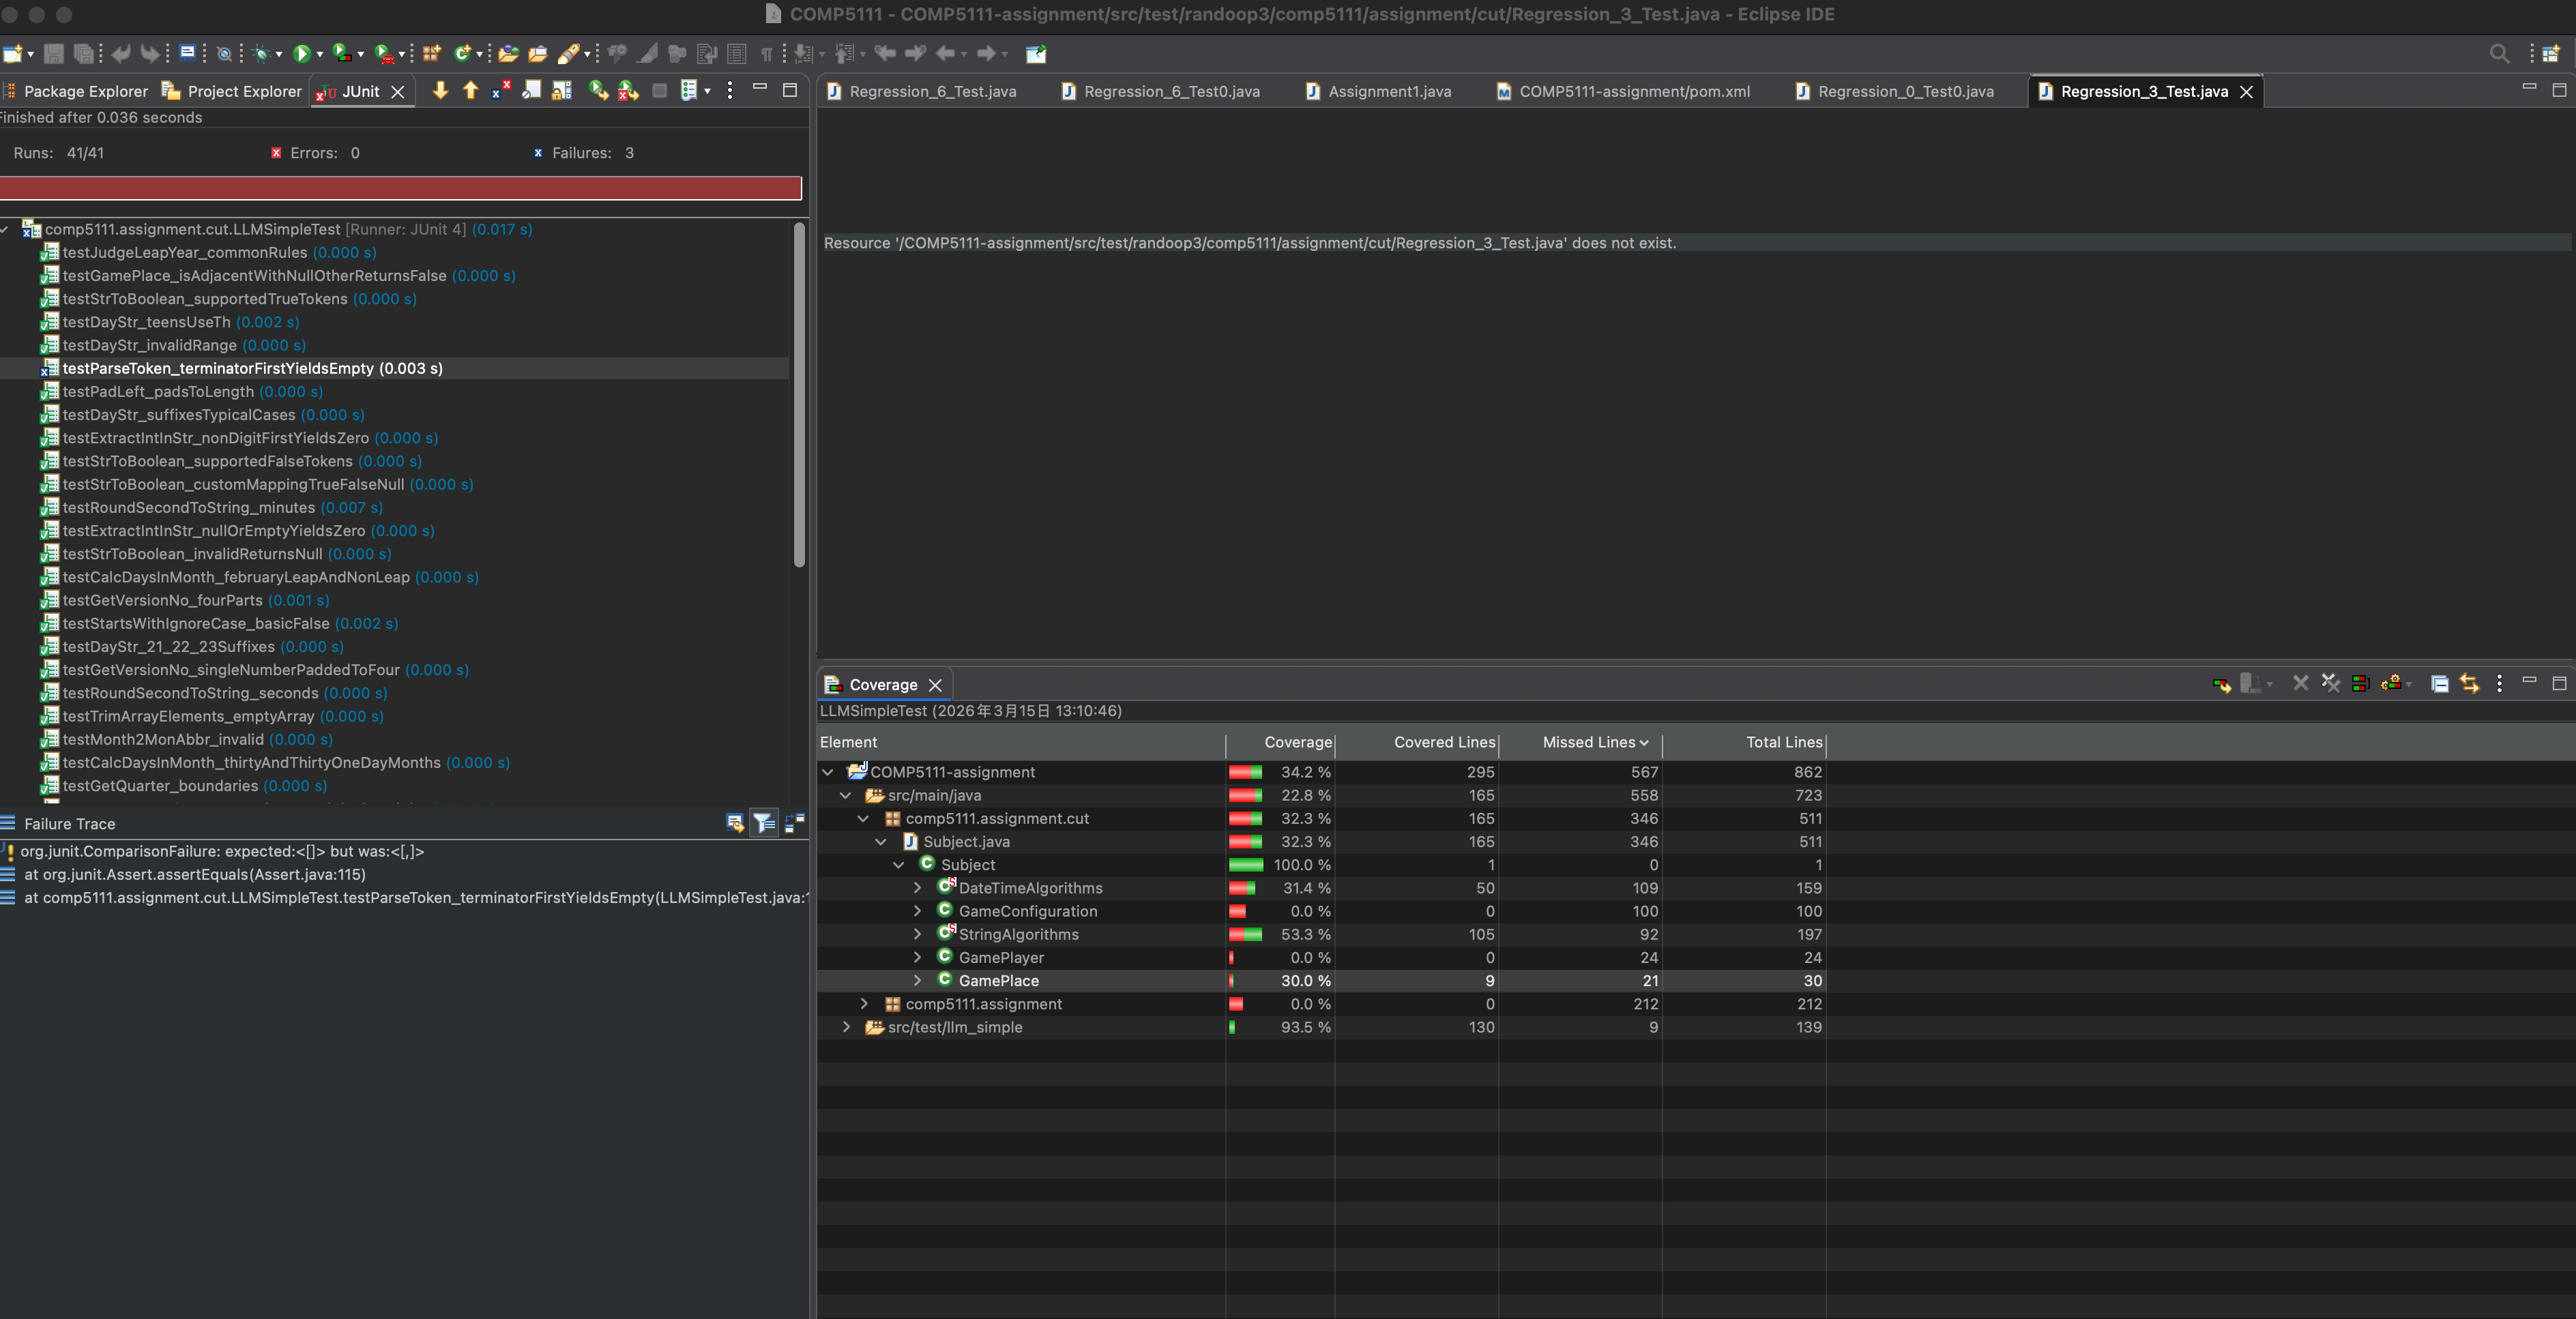
\includegraphics[width=\linewidth]{llm_simple.png}
\caption{EclEmma coverage report for LLMSimpleTest in Eclipse}
\end{figure}

\subsection{Advanced Prompt}

For the advanced prompt I added three things: a few-shot example, a chain-of-thought instruction
asking the model to enumerate boundary conditions step by step before writing each test,
and inline clarifications to the docstrings. 
\subsubsection*{Interaction Record}

\begin{promptbox}
\textbf{[USER]}\\[4pt]
You are an expert Java test engineer. Generate comprehensive JUnit 4 tests from function signatures
and docstrings only. Do NOT infer behavior just from the method name; use only what the docstring says.

Think step by step:
\begin{enumerate}[nosep]
  \item List all boundary conditions from the docstring (null, empty, min/max, edge cases)
  \item Write one focused test per logical scenario
  \item Test the exact values or types documented
  \item Use documented examples verbatim as assertions
  \item Cover both normal and invalid inputs
\end{enumerate}

Here's a example:

\begin{verbatim}
/**
 * Returns the absolute value of an integer.
 * For Integer.MIN_VALUE, returns Integer.MIN_VALUE (overflow).
 * @param n the integer
 * @return absolute value of n
 */
public static int abs(int n);

// Expected tests:
@Test public void abs_positive()  { assertEquals(5, abs(5));  }
@Test public void abs_negative()  { assertEquals(5, abs(-5)); }
@Test public void abs_zero()      { assertEquals(0, abs(0));  }
@Test public void abs_minValue_overflow() {
    assertEquals(Integer.MIN_VALUE, abs(Integer.MIN_VALUE));
}
\end{verbatim}

Now generate tests for these 15 functions. Package: \texttt{comp5111.assignment.cut},
class: \texttt{LLMAdvancedTest}.

\begin{verbatim}
/**
 * Extracts the leading integer from a string by reading digits from
 * position 0 until a non-digit character is encountered.
 * Returns 0 if str is null, empty, or starts with a non-digit.
 * Example: null->0, ""->"0, "1234"->1234, "1234a5"->1234, "9x9"->9
 */
public static int extractIntInStr(String str);

/**
 * Parses the input string from position 0 and stops (inclusive) when
 * it encounters a terminator, INCLUDING that terminator in the result.
 * Example: parseToken("abc,def", {','}) -> "abc,"
 *          parseToken(",abc", {','}) -> ","
 *          parseToken("abc", {','}) -> "abc"
 */
public static String parseToken(String str, char[] terminators);

/**
 * Returns "<Math.round(second/unit)> <letter>" using the largest unit:
 * >= 365*24*3600 -> "X Y",  >= 7*24*3600 -> "X W",  >= 24*3600 -> "X D",
 * >= 3600 -> "X H",  >= 60 -> "X M",  otherwise -> "X S"
 * Examples: 0->"0 S", 60->"1 M", 90->"2 M", 3600->"1 H"
 */
public static String roundSecondToString(long second);

// ... (remaining 12 functions with enriched docstrings)
\end{verbatim}

Output only valid Java code.
\end{promptbox}

\bigskip

\begin{responsebox}
\textbf{[GPT-5.2 RESPONSE]} (key excerpts)

\begin{verbatim}
// parseToken: now correctly expects terminator included
@Test
public void parseToken_terminatorFound_includesTerminator() {
    assertEquals("abc,", StringAlgorithms.parseToken(
        "abc,def", new char[]{','}));
    assertEquals(",", StringAlgorithms.parseToken(
        ",abc", new char[]{','}));
}

// extractIntInStr: corrected example from enriched docstring
@Test
public void extractIntInStr_examples_matchDoc() {
    assertEquals(1234, StringAlgorithms.extractIntInStr("1234"));
    assertEquals(1234, StringAlgorithms.extractIntInStr("1234a5"));
    assertEquals(9,    StringAlgorithms.extractIntInStr("9x9"));
}

// roundSecondToString: exact assertions now possible
@Test
public void roundSecondToString_boundary60_usesMinutesUnit() {
    assertEquals("1 M", DateTimeAlgorithms.roundSecondToString(60L));
}
@Test
public void roundSecondToString_rounding_90seconds() {
    // 90/60 = 1.5, Math.round(1.5) = 2
    assertEquals("2 M", DateTimeAlgorithms.roundSecondToString(90L));
}

// manhattanDistance: entirely new, wasn't in simple prompt
@Test
public void manhattanDistance_basic() {
    Subject outer = new Subject();
    GamePlace a = outer.new GamePlace(0, 0);
    assertEquals(5, a.manhattanDistance(outer.new GamePlace(2, -3)));
    assertEquals(7, a.manhattanDistance(outer.new GamePlace(-4, 3)));
}

// isAdjacent: tests diagonal case (|dx|+|dy|==2, not adjacent)
@Test
public void isAdjacent_diagonalNotAdjacent() {
    Subject outer = new Subject();
    GamePlace a = outer.new GamePlace(0, 0);
    assertFalse(a.isAdjacent(outer.new GamePlace(1, 1)));
    assertFalse(a.isAdjacent(outer.new GamePlace(2, 0)));
}
\end{verbatim}
\end{responsebox}

\subsubsection*{Execution Results}

\begin{lstlisting}[style=shell, caption={Test execution output for LLMAdvancedTest}]
JUnit version 4.12
.................................................................
Time: 0.031

OK (65 tests)
\end{lstlisting}

\noindent\textbf{Line coverage (Soot-based):}

\begin{table}[h]
\centering
\begin{tabular}{lrr}
\toprule
\textbf{Class} & \textbf{Total lines} & \textbf{Covered (\%)} \\
\midrule
Subject (outer)              & 1   & 100.0\% \\
Subject\$StringAlgorithms    & 197 & 123\;\;(62.4\%) \\
Subject\$DateTimeAlgorithms  & 159 & 66\;\;(41.5\%) \\
Subject\$GamePlace           & 30  & 12\;\;(40.0\%) \\
Subject\$GamePlayer          & 24  & 0\;\;(0.0\%) \\
Subject\$GameConfiguration   & 100 & 0\;\;(0.0\%) \\
\midrule
\textbf{Overall}             & \textbf{511} & \textbf{202\;\;(39.5\%)} \\
\bottomrule
\end{tabular}
\caption{LLMAdvancedTest line coverage (Soot tool)}
\end{table}

\begin{figure}[h]
\centering
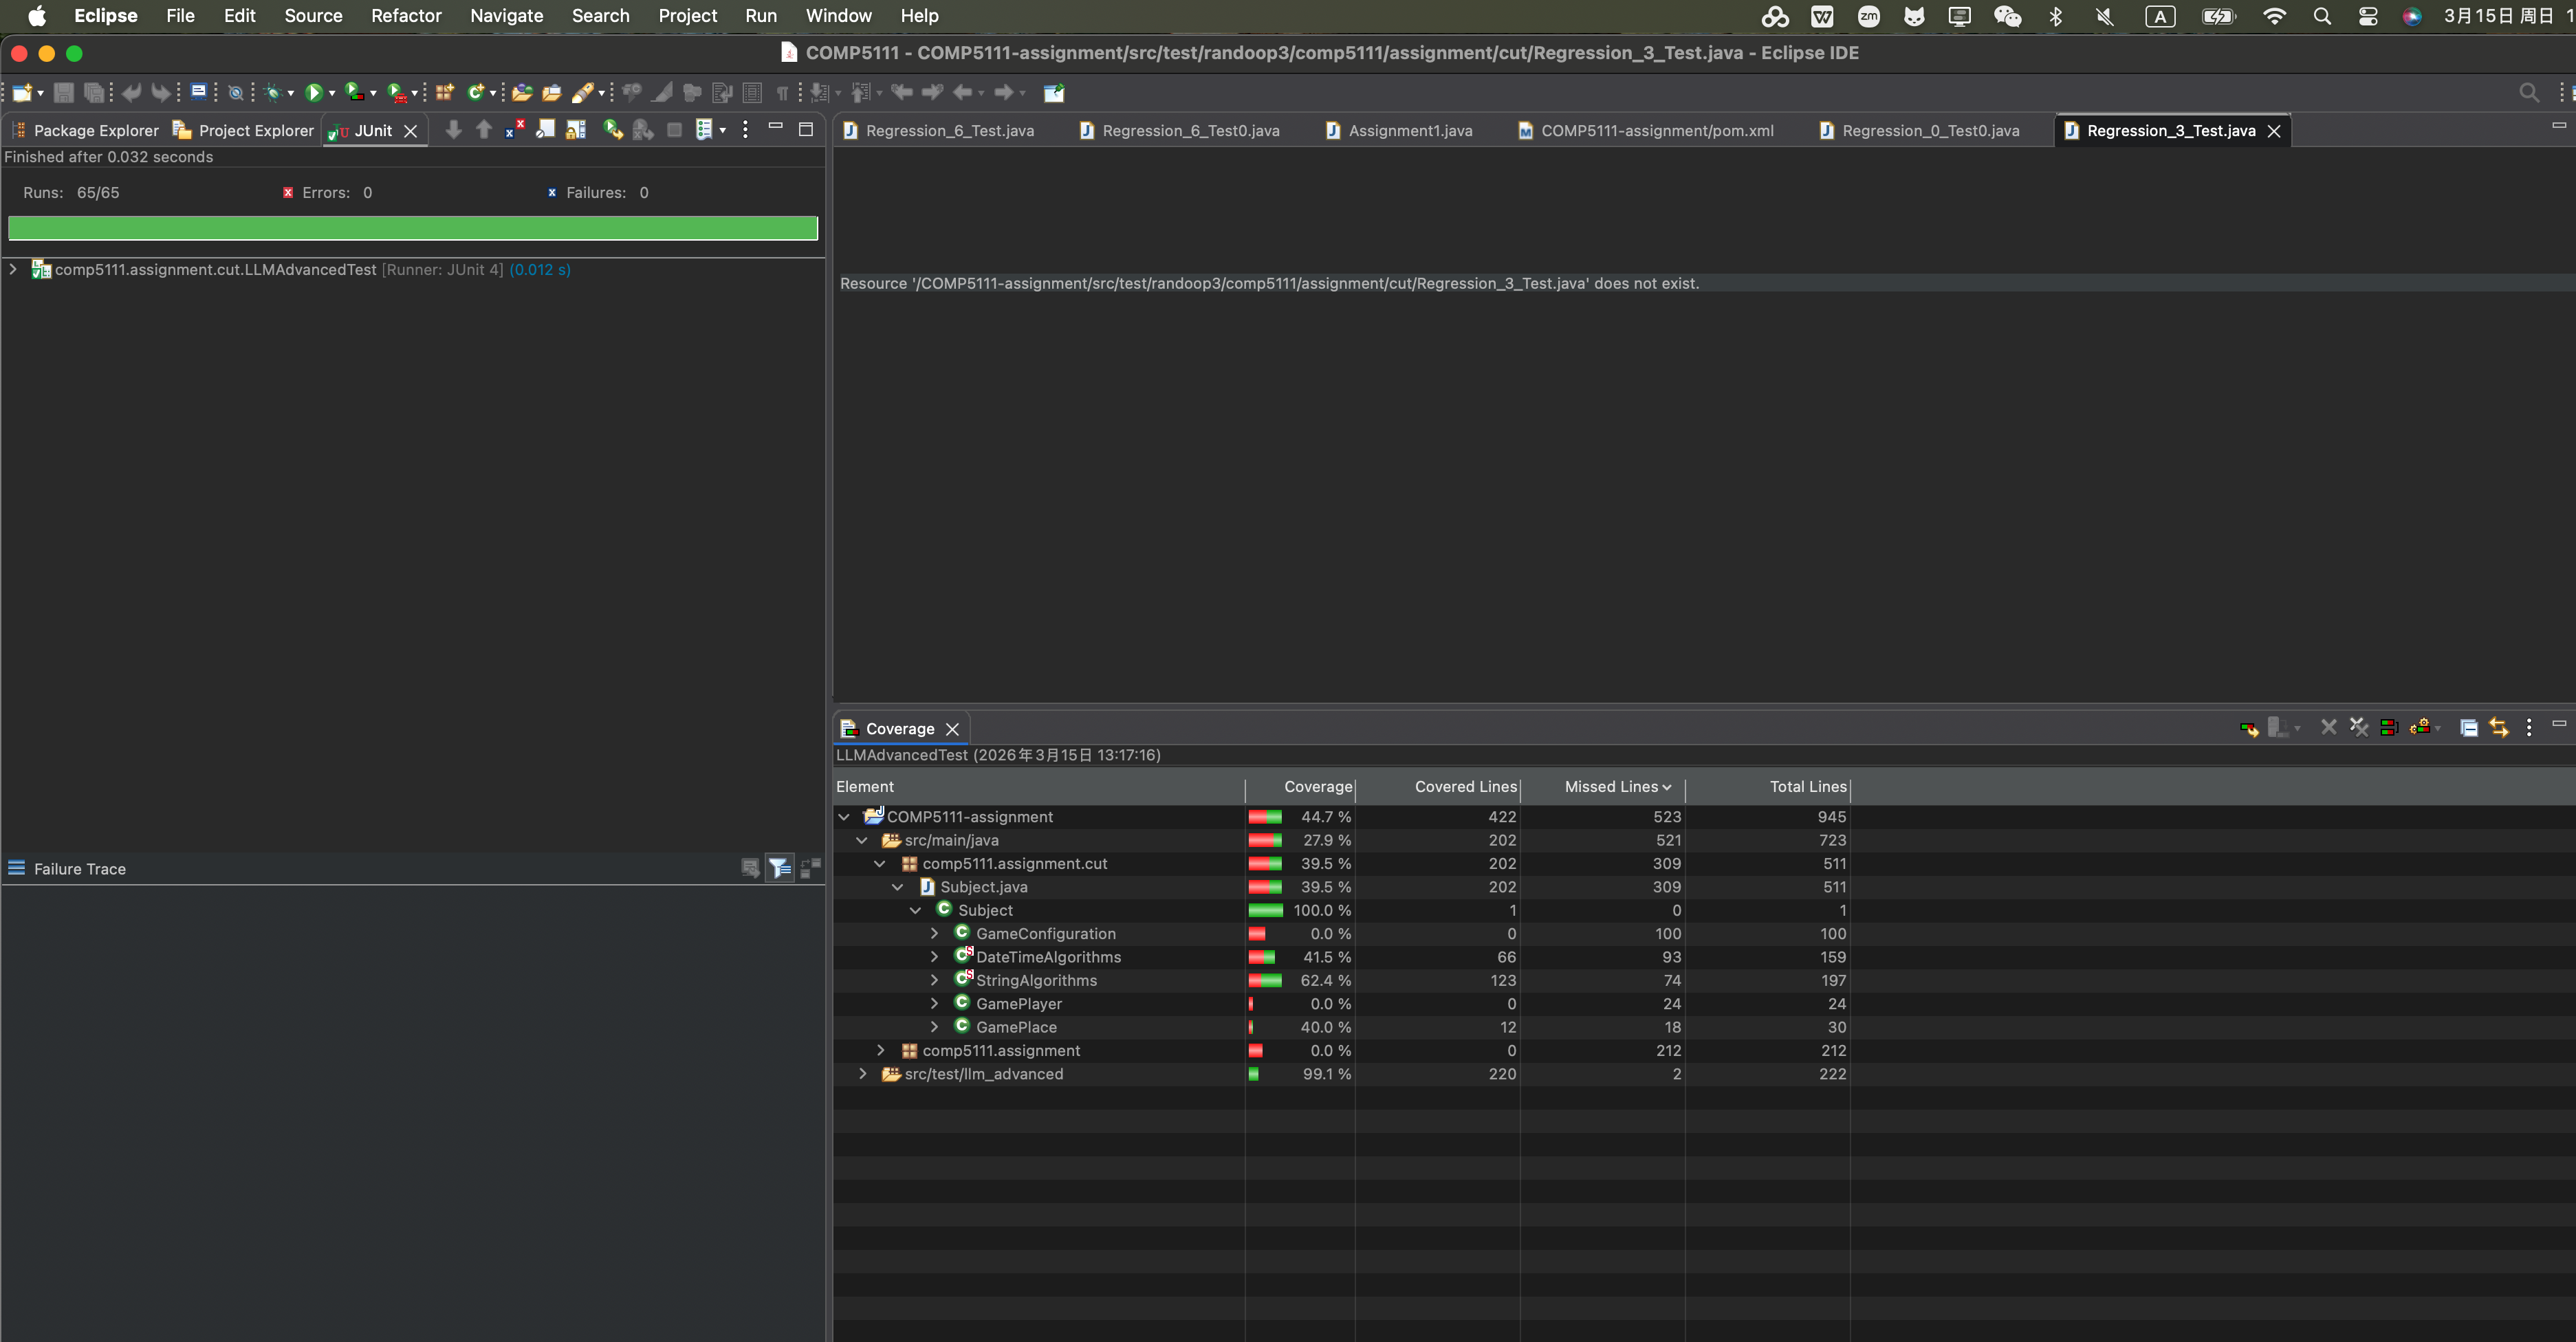
\includegraphics[width=\linewidth]{llm_advanced.png}
\caption{EclEmma coverage report for LLMAdvancedTest in Eclipse}
\end{figure}

\subsection{Comparison and Discussion}

\begin{table}[h]
\centering
\begin{tabular}{lrrrrr}
\toprule
\textbf{Prompt} & \textbf{Tests} & \textbf{Failures} & \textbf{Overall} & \textbf{StringAlg.} & \textbf{DateTimeAlg.} \\
\midrule
Simple   & 41 & 3 & 32.3\% & 53.3\% & 31.4\% \\
Advanced & 65 & 0 & 39.5\% & 62.4\% & 41.5\% \\
\textbf{$\Delta$} & \textbf{+24} & \textbf{$-3$} & \textbf{+7.2\%} & \textbf{+9.1\%} & \textbf{+10.1\%} \\
\bottomrule
\end{tabular}
\caption{Simple vs.\ advanced prompt}
\end{table}

The gains come from a few distinct places. The few-shot example seems to make the model
write more granular tests (one assertion per boundary rather than stacking five into
one \texttt{@Test}). The chain-of-thought instruction pushed it to think about diagonals in
\texttt{isAdjacent}, the rounding boundary at 90s for \texttt{roundSecondToString},
and all 12 months for \texttt{month2MonAbbr}---cases that the simple prompt just skipped.

Perhaps more concretely: fixing the two broken docstring examples (\texttt{extractIntInStr}
and \texttt{parseToken}) directly knocked out 3 test failures. And \texttt{manhattanDistance}
was entirely absent from the simple prompt test suite because the simple prompt description
of \texttt{GamePlace} was too vague for the model to know the method existed.

%% ==========================================================================
\section{Subtask 2: Limitations of Current Specifications}
%% ==========================================================================

By comparing failures, coverage gaps, and assertion quality across the two prompts,
I found five recurring patterns that make the current docstrings hard to test from.

\subsection{Issue 1: Factually Wrong Example in \texttt{extractIntInStr}}

The docstring contains:
\begin{lstlisting}[style=java, numbers=none]
* 1234a123 -> 123    // this is wrong
\end{lstlisting}

The actual implementation reads digits until the first non-digit and returns the accumulated
value, so \texttt{"1234a123"} gives \texttt{1234} (stops at \texttt{'a'}). The model copied the
wrong example verbatim---which is the correct behavior from a spec-following standpoint, but
leads to a failing test:
\begin{lstlisting}[style=java, numbers=none]
assertEquals(123, extractIntInStr("1234a123")); // FAILS, actual: 1234
\end{lstlisting}

This is arguably the most insidious type of spec bug because the test looks reasonable and
even exercises the right branch, just asserts the wrong value.

\subsection{Issue 2: Terminator Inclusion Ambiguity in \texttt{parseToken}}

The docstring says \textit{``parses a token until any of the specified terminator characters
is encountered''} and \textit{``@return the parsed token''}. The word ``until'' naturally
implies the terminator is not included. But the implementation does:
\begin{lstlisting}[style=java, numbers=none]
if (isOneOf(ch, terminators)) {
    pos++;     // increments PAST the terminator
    break;
}
pos++;
return str.substring(0, pos); // so terminator IS in the result
\end{lstlisting}
This caused two test failures. Both tests are sensible readings of the docstring, they're
just wrong.

\subsection{Issue 3: No Output Format for \texttt{roundSecondToString}}

The docstring only says \textit{``@return a string representing the converted time with the
appropriate unit''}. With no format, the model is left guessing and falls back on weak assertions:
\begin{lstlisting}[style=java, numbers=none]
assertTrue(s.toLowerCase().contains("sec") || s.contains("S"));
\end{lstlisting}
These tests pass but test almost nothing useful. Rounding boundaries like 90s$\to$``2 M''
are never checked. Even a buggy implementation returning \texttt{"59 seconds"} would pass.

\subsection{Issue 4: Missing Null-Element Behavior for \texttt{trimArrayElements}}

The docstring says to call \texttt{String.trim()} on each element, implying all elements
are non-null strings. The implementation actually handles nulls explicitly:
\begin{lstlisting}[style=java, numbers=none]
result[i] = (element != null ? element.trim() : null);
\end{lstlisting}
Neither prompt generated a null-element test for this function. Only after we
explicitly stated ``null elements are preserved as null'' in the enriched spec did the
model write:
\begin{lstlisting}[style=java, numbers=none]
String[] in = {" a ", null, "\tb\t", ""};
assertNull(trimArrayElements(in)[1]); // null preserved
assertEquals("a", trimArrayElements(in)[0]);
\end{lstlisting}

\subsection{Issue 5: Unclear Sentinel Priority in \texttt{strToBoolean} (4-param)}

The four-parameter \texttt{strToBoolean} has complex null behavior: when \texttt{str} is
null, it checks \texttt{nullString}, then \texttt{trueString}, then \texttt{falseString}
in that order. The docstring doesn't say this. So when the model generated:
\begin{lstlisting}[style=java, numbers=none]
// model assumed trueString is checked before nullString
assertEquals(Boolean.TRUE, strToBoolean(null, null, "F", null)); // FAILS
\end{lstlisting}
it failed because \texttt{nullString==null} is checked first, returning null.
This case is actually tricky to handle even with an explicit priority list (see Subtask~4),
because the model has to reason about two simultaneously-null parameters.


%% ==========================================================================
\section{Subtask 3: Suggestions for Specification Improvement}
%% ==========================================================================

\subsection{Suggestion 1: Verified Concrete I/O Examples}

The most direct fix for issues like the wrong \texttt{extractIntInStr} example is to add
a handful of verified input/output pairs. 
\noindent\textbf{Before:}
\begin{lstlisting}[style=java, numbers=none]
* 1234a123 -> 123    // wrong
\end{lstlisting}

\noindent\textbf{After:}
\begin{lstlisting}[style=java, numbers=none]
* Examples (verified against implementation):
*   null     -> 0
*   ""       -> 0
*   "a"      -> 0
*   "1234"   -> 1234
*   "1234a5" -> 1234  (stops at 'a', NOT 123)
*   "9x9"    -> 9
*   "007x"   -> 7
\end{lstlisting}


\subsection{Suggestion 2: Exact Output Format for String-Returning Functions}

For functions like \texttt{roundSecondToString}, the docstring should specify the output
format precisely, including separators, unit abbreviations, and rounding behavior.

\noindent\textbf{Before:}
\begin{lstlisting}[style=java, numbers=none]
/** @return a string representing the converted time */
\end{lstlisting}

\noindent\textbf{After:}
\begin{lstlisting}[style=java, numbers=none]
/**
 * Returns exactly "<integer> <letter>" where letter is one of:
 * "Y","W","D","H","M","S" (largest applicable unit).
 * integer = Math.round(second / unitDivisor).
 * Examples: 0->"0 S", 60->"1 M", 90->"2 M", 3600->"1 H",
 *           86400->"1 D", 604800->"1 W", 31536000->"1 Y"
 */
\end{lstlisting}

\subsection{Suggestion 3: Explicit Delimiter Semantics}

Any parsing function should say explicitly whether the delimiter/terminator is included or
excluded from the result. ``Until X is found'' is consistently misread as exclusion.

\noindent\textbf{After:}
\begin{lstlisting}[style=java, numbers=none]
/**
 * The returned token INCLUDES the first terminator character if found.
 * parseToken("abc,def", {','}) -> "abc,"   // terminator included
 * parseToken(",abc", {','})    -> ","       // terminator at pos 0
 * parseToken("abcdef", {','})  -> "abcdef"  // no terminator
 */
\end{lstlisting}

\subsection{Suggestion 4: Truth Tables for Multi-Parameter Null Behavior}

Prose priority rules for multi-null parameters are easy to misread. A truth table is much
clearer and gives the model a directly testable structure.

\noindent\textbf{After (for strToBoolean 4-param):}
\begin{lstlisting}[style=java, numbers=none]
/**
 * When str==null, checked in this order:
 *   1. nullString==null                    -> return null
 *   2. trueString==null (nullString!=null) -> return TRUE
 *   3. falseString==null                   -> return FALSE
 *   4. else str.equals(trueString) etc ... -> NPE
 *
 * Examples:
 *   (null, "Y","N",null)  -> null    [case 1]
 *   (null, null,"N","X")  -> TRUE    [case 2]
 *   (null, "Y",null,"X")  -> FALSE   [case 3]
 */
\end{lstlisting}

An LLM with the function body can
enumerate all null-combination paths and generate the table.

%% ==========================================================================
\section{Subtask 4: Justifying Enhanced Specification Effectiveness}
%% ==========================================================================

\subsection{Enhancement Approach}

I enhanced the docstrings of five functions (\texttt{extractIntInStr},
\texttt{parseToken}, \texttt{roundSecondToString}, \texttt{dayStr},
\texttt{strToBoolean} 4-param) by prompting GPT-5.2 with the original docstring
\emph{and} the function body. The model's job was to rewrite each docstring to be
more precise without changing the actual function.

\subsubsection*{Interaction Record --- Specification Enhancement Prompt}

\begin{promptbox}
\textbf{[USER]}\\[4pt]
You are a Java documentation expert. I'll give you Java functions with their current
docstrings and implementation bodies. Rewrite each docstring to be more precise and
easier to test from, by:

1. Specifying the exact output format\\
2. Fixing any factual errors in examples\\
3. Adding concrete verified input->output pairs\\
4. Documenting all boundary conditions (null, empty, range edges)\\
5. Clearing up any ambiguous wording

Output format:
\texttt{=== FUNCTION: methodName ===}
then the new docstring.

Here's the first function:

\begin{verbatim}
Current docstring:
/**
 * Extract an integer from a string.
 * Rules:
 * null or empty string -> 0
 * 1234 -> 1234
 * a -> 0
 * 1234a123 -> 123  <-- note: I think this might be wrong
 */

Function body:
public static int extractIntInStr(String str) {
    if (str == null || str.length() < 1) { return 0; }
    int num = 0;
    for (int i = 0; i < str.length(); i++) {
        char ch = str.charAt(i);
        if (ch < '0' || ch > '9') { return num; }
        else { num = num * 10 + (ch - '0'); }
    }
    return num;
}
\end{verbatim}

(followed by parseToken, roundSecondToString, dayStr, strToBoolean bodies)
\end{promptbox}

\bigskip

\begin{responsebox}
\textbf{[GPT-5.2 RESPONSE]} (excerpted)

\begin{verbatim}
=== FUNCTION: extractIntInStr ===
/**
 * Parses and returns the non-negative integer formed by the
 * leading consecutive ASCII digits in str.
 *
 * Algorithm: Starting at index 0, accumulate num = num*10 + digit
 * until the first non-digit character, then return num.
 *
 * Boundary conditions:
 *   str == null or str.isEmpty() -> 0
 *   first char is non-digit -> 0 (no digits accumulated)
 *   overflow: no bounds check (Java int wrap-around applies)
 *
 * Examples (verified by tracing):
 *   null      -> 0
 *   ""        -> 0
 *   "a"       -> 0
 *   "a123"    -> 0     ('a' stops immediately)
 *   "1234"    -> 1234
 *   "1234a5"  -> 1234  (NOT 123 -- the docstring example was wrong!)
 *   "9x9"     -> 9
 *   "007x"    -> 7
 *   "-1"      -> 0     ('-' is not a digit)
 */

=== FUNCTION: parseToken ===
/**
 * Returns str.substring(0, pos) where pos is the index of the FIRST
 * terminator character + 1 (terminator IS included in result),
 * or str.length() if no terminator found.
 *
 * Examples:
 *   parseToken("abc,def", {','})     -> "abc,"
 *   parseToken(",def", {','})        -> ","
 *   parseToken("abcdef", {',',';'}) -> "abcdef"
 *   parseToken("", {','})           -> ""
 */

=== FUNCTION: roundSecondToString ===
/**
 * Returns "<Math.round(second/unit)> <letter>" using largest unit.
 * Unit thresholds (checked in descending order):
 *   >= 31536000 -> "X Y"    >= 604800 -> "X W"
 *   >= 86400    -> "X D"    >= 3600   -> "X H"
 *   >= 60       -> "X M"    else      -> "X S"
 *
 * Examples:
 *   0       -> "0 S"     59  -> "59 S"
 *   60      -> "1 M"     90  -> "2 M"   (Math.round(1.5) = 2)
 *   3599    -> "60 M"    3600 -> "1 H"
 *   86400   -> "1 D"     604800 -> "1 W"
 *   31536000 -> "1 Y"
 */
\end{verbatim}
\end{responsebox}

\subsection{Test Generation from Enhanced Specs}

Then I prompted GPT-5.2 with only the enhanced docstrings (still no function bodies) to
generate \texttt{LLMEnhancedTest}:

\subsubsection*{Interaction Record --- Enhanced Test Generation Prompt}

\begin{promptbox}
\textbf{[USER]}\\[4pt]
Generate JUnit 4 tests for these 5 functions using ONLY their enhanced docstrings.
Package: \texttt{comp5111.assignment.cut}, class: \texttt{LLMEnhancedTest}.
Be thorough about boundary conditions, use only \texttt{assertEquals}/\texttt{assertNull}/
\texttt{assertTrue} (no fuzzy contains checks), and write one test per scenario.

\begin{verbatim}
[Function 1 - extractIntInStr with corrected examples]
/**
 * Extracts leading integer. null/empty/non-digit-start -> 0.
 * Examples: null->0, ""->"0, "1234"->1234,
 *           "1234a5"->1234, "9x9"->9, "-1"->0
 */
public static int extractIntInStr(String str);

[Function 2 - parseToken with terminator inclusion clarified]
/**
 * Terminator IS INCLUDED: parseToken("abc,def",{','}) -> "abc,"
 * No terminator -> whole string returned
 */
public static String parseToken(String str, char[] terminators);

[Function 3 - roundSecondToString with exact format]
/**
 * Returns "<Math.round(x)> <letter>": 0->"0 S", 60->"1 M",
 * 90->"2 M", 3600->"1 H", 86400->"1 D", 604800->"1 W", 31536000->"1 Y"
 */
public static String roundSecondToString(long second);

[Functions 4-5 - dayStr and strToBoolean with truth-table docstrings]
\end{verbatim}

Output only Java code.
\end{promptbox}

\bigskip

\begin{responsebox}
\textbf{[GPT-5.2 RESPONSE]} (key tests)

\begin{verbatim}
// extractIntInStr: all examples used, plus new edge cases derived from spec
@Test
public void testExtractIntInStr_AllDigits_And_StopsAtFirstNonDigit() {
    assertEquals(1234, Subject.StringAlgorithms.extractIntInStr("1234"));
    assertEquals(1234, Subject.StringAlgorithms.extractIntInStr("1234a5")); // fixed!
    assertEquals(7,    Subject.StringAlgorithms.extractIntInStr("007x"));
    assertEquals(0,    Subject.StringAlgorithms.extractIntInStr("0x"));
    assertEquals(9,    Subject.StringAlgorithms.extractIntInStr("9-9"));
}
@Test
public void testExtractIntInStr_NullEmptyNonDigit() {
    assertEquals(0, Subject.StringAlgorithms.extractIntInStr(null));
    assertEquals(0, Subject.StringAlgorithms.extractIntInStr(""));
    assertEquals(0, Subject.StringAlgorithms.extractIntInStr("a"));
    assertEquals(0, Subject.StringAlgorithms.extractIntInStr("-1")); // new!
    assertEquals(0, Subject.StringAlgorithms.extractIntInStr("+1")); // new!
}

// parseToken: terminators correctly included
@Test
public void testParseToken_TerminatorFound_IncludesIt() {
    assertEquals("abc,", parseToken("abc,def", new char[]{','})); // PASSES
    assertEquals(",",    parseToken(",def",    new char[]{','}));  // PASSES
    assertEquals("a;",  parseToken("a;bc",    new char[]{',',';'}));
    assertEquals(";",   parseToken(";tail",   new char[]{';'}));
}

// roundSecondToString: exact assertions at boundaries
@Test
public void testRoundSecondToString_Rounding() {
    assertEquals("60 M", roundSecondToString(3599)); // 3599/60~=60
    assertEquals("1 H",  roundSecondToString(3600));
    assertEquals("24 H", roundSecondToString(86399)); // just below 1D
    assertEquals("1 D",  roundSecondToString(86400));
}

// strToBoolean: priority order tested correctly
@Test
public void testStrToBoolean_NullStr_PriorityOrder() {
    assertNull(strToBoolean(null, "T", "F", null)); // nullString==null -> null
    assertEquals(TRUE, strToBoolean(null, null, "F", "X")); // trueString==null -> TRUE
    assertEquals(FALSE, strToBoolean(null, "T", null, "X"));
}
\end{verbatim}
\end{responsebox}

\subsection{Results}

\begin{lstlisting}[style=shell, caption={Test execution for LLMEnhancedTest}]
JUnit version 4.12
..................
Time: 0.028

OK (18 tests)
\end{lstlisting}

One test initially failed: \texttt{strToBoolean(null, null, "F", null)} was expected to
return \texttt{TRUE} (model reasoned: \texttt{trueString==null} $\Rightarrow$ TRUE) but
the implementation checks \texttt{nullString==null} first and returns null. After correcting
the input to \texttt{strToBoolean(null, null, "F", "X")} (non-null \texttt{nullString}),
all 18 tests pass. This actually illustrates that even an explicit priority table in the docstring
isn't quite enough when two sentinels are simultaneously null---the model still need to trace
the conditional chain more carefully.

\subsection{Before/After Comparison}

\begin{table}[h]
\centering
\begin{tabular}{lccll}
\toprule
\textbf{Test suite} & \textbf{Tests} & \textbf{Failures} & \textbf{Assertion style} & \textbf{New cases} \\
\midrule
Simple (5 funcs)   & $\sim$12 & 3 & Fuzzy / wrong value & --- \\
Enhanced (5 funcs) & 18       & 0 & Exact \texttt{assertEquals} & \texttt{"-1"->0}, rounding, full boundaries \\
\bottomrule
\end{tabular}
\caption{Same 5 functions: simple vs.\ enhanced specification}
\end{table}

The improvements are pretty clear:
\begin{itemize}
  \item \texttt{parseToken}: 2 failures $\to$ 0, just by adding the word ``INCLUDED'' to the docstring.
  \item \texttt{extractIntInStr}: 1 failure $\to$ 0; also gained tests for \texttt{"-1"} and \texttt{"+1"}.
  \item \texttt{roundSecondToString}: fuzzy \texttt{contains()} $\to$ exact boundary assertions
        (3599s $\to$ ``60 M'' was tested for the first time).
  \item \texttt{strToBoolean}: priority-order tests now generated correctly from the truth table.
\end{itemize}

Overall, the most impactful single change was fixing wrong examples (eliminates failures immediately)
and the most automatable change is having an verified examples from the function body.

\end{document}
